%!TEX root = main.tex

% =============================================================================
\section{Background on LSM Trees}
\label{sec:background}
% =============================================================================



\Paragraph{Basics} 
LSM trees use the \textit{out-of-place} ingestion paradigm to store key-value
pairs. Writes, updates, or deletes are buffered in a memory buffer, and once
full, its contents are sorted based on the key, forming an
\textit{immutable sorted run}. This run is then flushed to the first level on
secondary storage. Each level of sorted runs has a maximum permitted size, which
is tunable. Overall, for an LSM tree with $L$ disk-resident levels, we denote the
memory buffer as Level $0$, and the remaining
levels in storage, level $1$ to $L$. The disk-resident sorted runs have exponentially increasing
sizes following a tunable size ratio $\sizeratio$.
Figure \ref{fig:lsm-overview} shows an overview of an LSM tree.

\begin{figure}[h]
    \centering
    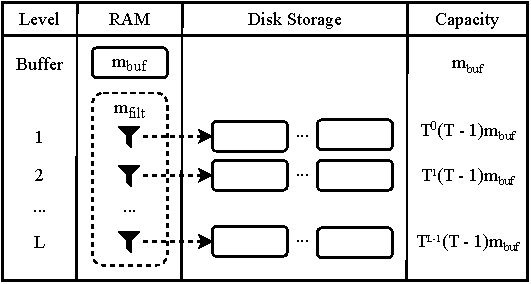
\includegraphics[scale=0.75]{figures/lsm_overview.pdf}
    \caption{Overview of the structure of an LSM tree}
    \label{fig:lsm-overview}
\end{figure}


We denote the number of bits of main memory allocated to the buffer as $\mbuf$,
which holds a number of entries with fixed entry size $E$. For example, in
RocksDB the default buffer size is $\mbuf=64$MB, and depending on the
application, the entry size typically varies between 64B and 1KB. 

Level 0 can be updated in-place since it is in memory, however, the runs in
levels 1 and beyond are immutable. Each Level $i$ has a capacity threshold of
$(\sizeratio - 1) T^{i-1} \cdot \frac{\mbuf}{E}$ entries , thus, levels have
exponentially increasing capacities by a factor of $\sizeratio$.  The total
number of levels $L$ for a given {\sizeratio} is 

\begin{equation} 
L(T) = \Bigg\lceil \log_T \left( {\frac{N \cdot E}{\mbuf}} + 1 \right) \Bigg\rceil ,
\label{eq:levels}
\end{equation}

where $N$ is the total number of physical entries across all levels including
updates and deletions \cite{Dayan2018a, Luo2020, Sarkar2020}. 


\Paragraph{Compaction Policies: Leveling and Tiering} 
Classically, LSM trees support two merging policies: leveling and tiering. 
In leveling, each level may have at most one run, and every time a run in Level
    $i - 1$ ($i \geq 1$) is moved to Level $i$, it is greedily sort-merged
    (compaction) with the run from Level $i$, if it exists. 
With tiering, every level must accumulate $\sizeratio$ runs before they trigger
    a compaction. 
During a compaction, entries with a matching key are consolidated and only the
    most recent valid entry is retained~\cite{Dong2017, ONeil1996}. 
Recently hybrid compaction policies fuse leveling and tiering in a single tree
    to strike a balance between the read and write throughput~\cite{Dayan2018,
    Dayan2019}.


\Paragraph{LSM tree Operations}
An LSM tree supports: (a) writes of new key-value pairs, (b) point queries, or
(c) range queries.

\emph{Writes:} A write operation is handled by a buffer append, and if the
buffer gets full, it triggers a compaction as discussed above. Any write may
include either a new key-value pair, a key-value pair that invalidates an
existing one (an \emph{update}), or a special key-value pair that deletes an
existing one (a \emph{delete}).


\emph{Point Queries:}
A point query searches for the value of a specific unique key. It begins by
looking at the memory buffer, then traverses the tree from the smallest level to
the largest one. For tiering, within a level, a lookup moves from the most to
the least recent tier. The lookup terminates when it finds the first matching
entry. Note that a point query might return an \emph{empty} result or a
\emph{non-empty} result. We differentiate the two because, in general, workloads
with empty point queries can be further optimized \cite{Dayan2017,Dayan2018a}.

\emph{Range Queries:}
A range lookup returns the most recent versions of the target keys 
by sort-merging the qualifying key ranges across all runs in the tree.

\Paragraph{Optimizing Lookups} 
Read performance is optimized using Bloom filters and fence pointers. 
In the worst case, a lookup 
needs to probe every run. To reduce this cost, 
LSM engines use one Bloom filter per run in main memory~\cite{Dayan2017, FacebookRocksDB}. 
Bloom filters \cite{Bloom1970} are probabilistic membership test data structures
    that exhibit a false positive $f$ as a function of the ratio between the
    memory allocated $\mfilt$ to them and the elements it indexes.
In LSM trees, Bloom filters allow a lookup to skip probing a run altogether if
    the filter-lookup returns negative.
In practice, for efficient storage, Bloom filters are maintained at the
    granularity of files~\cite{Dong2017}. 
Fence pointers store the smallest key per disk page in memory~\cite{Dayan2017},
    to quickly identify which page(s) to read for a lookup, and perform up to
    one I/O per run for point lookups.


\Paragraph{Tuning LSM Trees} 
Prior to this work, efforts to systematically tune LSM trees assume that the
    workload information and the environmental setup is accurately known.
Under that assumption, the main focus on LSM tuning has been on deciding how to
allocate the available main memory between Bloom filters and buffering
\cite{Dayan2017,Kim2020,Luo2020a}, while often the size ratio and the merging
strategy was also co-tuned \cite{Dayan2018a}.  In addition, recent work has
introduced new hybrid merging strategies \cite{Dayan2018,Dayan2019,Sarkar2021c},
and optimizations for faster data ingestion \cite{Luo2019b} and performance
stability
\cite{Luo2019a}.

